\chapter{Preparation}\label{preparation}

\ifpdf
    \graphicspath{{Chapter2/Figs/Raster/}{Chapter2/Figs/PDF/}{Chapter2/Figs/}}
\else
    \graphicspath{{Chapter2/Figs/Vector/}{Chapter2/Figs/}}
\fi



\section{Balls-into-Bins}


The simple balls-into-bins models have been introduced in the 20th century as probability theory problems under several different names, e.g. ``urn processes'' or ``occupancy problems'' \cite{kolchin1978coined}. A few years later its applicability to real world problems, such as load balancing, has been highlighted, and further research led to the analyses of even more realistic and efficient models. Apart from practical applications, the results derived for balls-into-bins models turned out to be useful in the analysis of several other (randomised) algorithms \cite{edmonds2006cakecutting}. It is still an actively researched field gaining much attention, and in particular, the main model I will study has been first analysed theoretically in 2019 \cite{dwivedi2019firstthinning}.


\subsection{Definitions and Assumptions}



The real-world load balancing problem is very complex, and the exact characteristics differ between cases. For example, the servers might (or might not) be different (e.g. they serve different types of requests, or they just have different speed), the arrival rate of the jobs might be unknown (or maybe an estimated model is possible), servers might crash, etc. Building a theoretical model that is completely general and can still be analysed effectively seems infeasible. Hence, most of the balls-into-bins models capture one or a few characteristics of load balancing, and therefore they are very diverse. There are however some common assumptions that all of models that I study make. Next I present a sufficiently general definition of the balls-into-bins abstraction, and state its assumptions. 

\begin{definition}[Balls-into-bins] \label{definition: balls-into-bins}
In the balls-into-bins problems, there are $n$ bins, and there are $m$ balls arriving sequentially. Whenever a ball arrives, it is placed in one of the bins according to a randomised protocol.
\end{definition}


Here are the most important assumptions made by the balls-into-bins model:


\begin{itemize}
    \item
    Balls never leave the bins. While in most real-world scenarios jobs do end, this model can still provide a good local approximation, or represent the overall work assigned over a time period. Also, most of the theoretical works in the literature analyse the normalised (maximum) load, i.e. the difference between the (maximum) load and the average load over all the servers, and this subtraction has a similar type of effect as finishing jobs over time \NOTE{A}{This is very creative and it is my own idea, check if it makes any sense or maybe should explain some more.}. For other applications, such as hashing \cite{udi2017ballsintobinslandscape}, persistent balls are realistic. There are nevertheless some balls-into-bins settings that include also the deletion of the balls \cite{azar1999twochoice}, but I will not consider those in this dissertation.
    \item
    The number of balls $m$ is known in advance. As shown in \cite{feldheim2021longtermthinning}, there are much better performing protocols with this assumption (in terms of normalised maximum load). In many applications, even if $m$ is unknown, it can be estimated from previous runs (e.g. days).
    \item
    The balls and the bins are homogeneous. This assumes that there is just a single type of job (e.g. they are of unit size) and all the servers are of the same quality (e.g. they have the same speed). These assumptions are valid in several cases, e.g. even though Google searches are different, a built-in timeout mechanism makes them approximately unit-sized \NOTE{A}{Reference?}. The more general case of heterogeneous balls and bins has also been analysed, see e.g. \cite{berenbrink2008weighted}.
    \item
    The randomised protocols are assessed according to the expected value of maximum load after all $m$ balls have been allocated (\textbf{expected final maximum load}). Even though (expected) normalised (final) maximum load is the most widespread objective in the literature, I found it simpler to present the results with the raw maximum load, and the optimisation objective is not affected by this (the difference is just a constant $\frac{m}{n}$). It is important to emphasize the stochastic nature of the process, that is why we optimise an expected value. Note that while there are several other metrics that can be important for load balancing in practice (e.g. expected empirical variance of the final loads, variance of final maximum load, expected maximum normalised load throughout the whole run), only a few papers have considered those so far \cite{feldheim2021longtermthinning}, so I do not discuss them any further. \NOTE{A}{Should I expand more on what the varience of the load distribution, the variance of the maximum load etc. mean?}
    
\end{itemize}





\subsection{Settings} \label{settings}

In this section I will define the randomised protocols that I will study in later chapters. Note that in the literature when a protocol such as \TwoThinning is discussed, they often use the term (\TwoThinning) ``setting'', referring more generally to the full context of balls-into-bins with that protocol. I will also adapt this terminology.


\iffalse % I don't think this paragraph is needed
The general pattern in the protocols below is that they are more robust and are easier to implement than deterministic protocols (as discussed in Chapter \ref{introduction}), and some of them still provide sufficient guarantees on the objective function (maximum load). The theoretical analysis of the protocols according to the objective function is deferred until Chapter \ref{evaluation}.
\fi

\paragraph{\OneChoice}

This is the simplest randomised algorithm. The arriving ball is allocated uniformly at random into one of the bins.

\paragraph{\TwoChoice}
\NOTE{T}{I would prefer a more concise, mathematical description of each protocol, clearly separated from motivation etc. Andor: I agree it would be nice, but I am not sure if it is worth the effort to set up some notation, as I don't use it later.}
In this setting, two bins are chosen uniformly at random (possibly the same two bins), and the ball is placed in the lesser loaded of the two bins . In case of a tie, the ball is allocated uniformly at random into one of the two bins. Implementing \TwoChoice in practice is challenging due to concurrency and communication delays: the servers need to report their loads by interrupting their currently running process; the client has to wait for the response by both servers, and then allocate the job to one of them (one and half round trips).

A generalisation of \TwoChoice is \KChoice, where not $2$, but $K$ bins are compared - I do not discuss it any further, since it has been shown to provide only minor improvement in terms of the maximum load over \TwoChoice \cite{azar1999twochoice}.


\paragraph{\TwoThinning}

This is one of the main settings I will focus on, and this has been defined in Chapter \ref{introduction} already.

\iffalse %I should double check, but I think this is all explained in the fst chapter. 
. Here I present the main interpretation of this protocol, but in Section\NOTE{T}{Section} \ref{alternative} I present another way to look at this setting. An important difference between this protocol, and \KChoice is that this protocol additionally requires a decision strategy, a free parameter of the protocol\NOTE{D}{Maybe remove ``a free parameter of the protocol''}. When a ball arrives, a (primary) bin is chosen uniformly at random, and the according to the strategy, the primary bin is accepted, and the ball is placed into that bin, or it is rejected, and the ball is placed into a (secondary) bin chosen again uniformly at random. \NOTE{D}{This strategy is commonly a threshold function.}The motivation for this interpretation of \TwoThinning is that unlike for \TwoThinning\NOTE{D}{Two-Choice?} where always $2$\NOTE{D}{two} servers are interrupted by a query, here if the primary load is accepted by the strategy, than only $1$\NOTE{D}{one} server is interrupted. A subtlety is that the secondary and primary bins can in fact be the same, while in a real-world application, the client would probably avoid the primary bin if it has been rejected\NOTE{D}{OK, but the improvement is minor}.
\fi

\paragraph{\KThinning}

\KThinning is a generalisation of \TwoThinning, just like \KChoice for \TwoChoice. Whenever a ball arrives, up to $k$ bin samples are taken sequentially uniformly at random until one of them is accepted by the decision strategy, and that is the bin where the ball is placed. Unlike for the \KChoice generalisation, this generalisation does provide a major improvement \cite{feldheim2020dthinning} \cite{los2021quantilethreshold}.


\paragraph{\GraphicalTwoChoice}

\NOTE{D}{This paragraph is quite long. Try to untangle into (1) model definition and practicality and (2) What you have achieved (although this might be better suited for the next section)}
This setting is a generalisation of \TwoChoice, where not all pairs of bins can be sampled. Instead, treating the bins as nodes and the pairs that can be sampled as edges of a graph, \GraphicalTwoChoice samples an edge uniformly at random for each ball. Note that remarkably, the greedy strategy, that allocates the ball into the lesser loaded of endpoint of the edge has been shown not to be optimal in general, and hence this setting also requires a decision strategy. I present the first known concrete counterexample for the suboptimality of Greedy in Lemma \ref{lemma: greedy-suboptimal}. It is often assumed that the graph is regular (i.e. all nodes have the same degree), otherwise the symmetric final maximum load objective function is not reasonable -- take the star graph as an example of a highly unbalanced graph  \NOTE{A}{How to cite it properly?}.

\begin{figure}[hbt!] \label{star-graph}
    \centering
    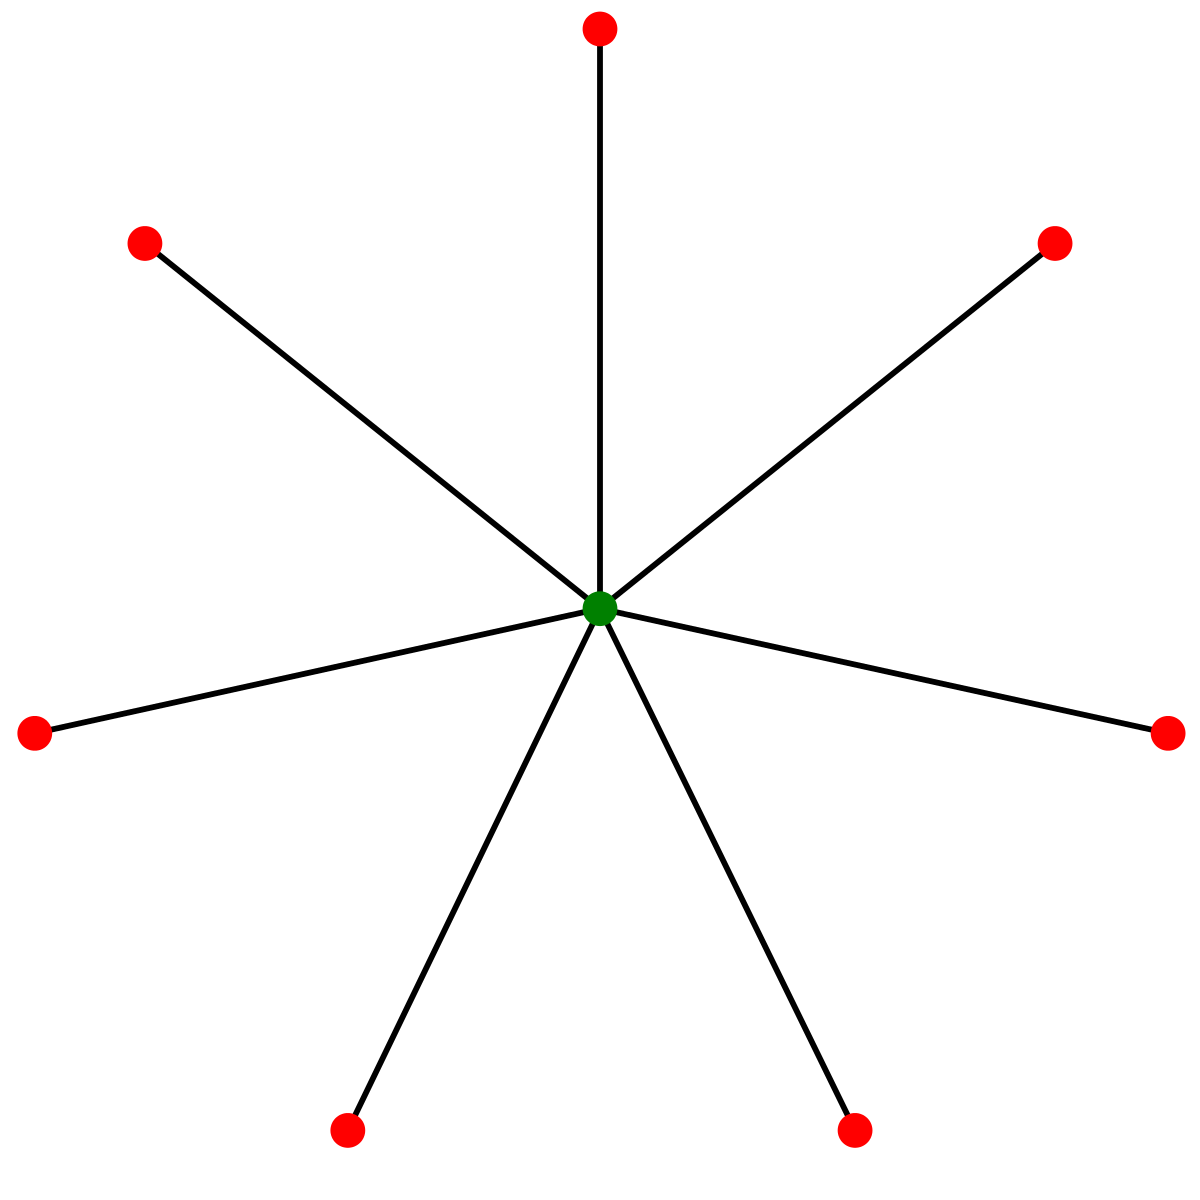
\includegraphics[scale=0.1]{Chapter2/Figs/star_graph.png}
    \caption{Star graph \cite{stargraph}}
\end{figure}


The real-world motivation for this setting stems from the geographical locality of the servers. One possible practical implementation of \GraphicalTwoChoice for load balancing could be that the client chooses a server $A$ uniformly at random, server $A$ queries the exact current load of a neighbouring server $B$ uniformly at random, and then $A$ decides whether itself or $B$ should complete the job. In this case the edges correspond to nearby servers, but different underlying graphs are also possible \cite{peres2015oneplusbeta}. For this dissertation, I will make the same simplifying assumptions for \GraphicalTwoChoice as for \TwoThinning. \NOTE{A}{Should I explain more?}


Analogously, \textsc{Graphical Two-Thinning} is a reasonable protocol as well, but I chose to focus on \GraphicalTwoChoice, since there is more literature available on that, and hence a more thorough comparative evaluation is possible.\\


\iffalse
As stated briefly in Chapter \ref{introduction}, the project is about optimising free parameters of various balls-into-bins settings. Now with the definitions in hand, we can see that it amounts to finding good strategies for \TwoThinning, \KThinning and \GraphicalTwoChoice. While most of the available strategies are manually defined (e.g. choose the lesser loaded, or accept if greater than $x$), I will use algorithms to find good strategies! Hence, I would like to make an important distinction between \textbf{protocol}\NOTE{T}{better to use always protocol, and not setting. Otherwise too many terms...} and \textbf{algorithm}: an algorithm is used to optimise free parameters of a protocol, which can then be used in the balls-into-bins framework with the parameters generated by the algorithm. In particular, I will use RL and dynamic programming as algorithms, to find good strategies for the parametric protocols discussed above. I will use this terminology from now on. On this note, I will use the terms \textbf{decision strategy} and the more general term \textbf{free parameters} interchangeably, always choosing based on the context. \NOTE{A}{Move elsewhere?}\NOTE{D}{Maybe somewhere with the subheading ``notation''}
\fi

\subsection{Notes on Related Work and Background Reading}

\NOTE{A}{Give more concrete examples?!}

As part of the preparation I was reading several papers about the theory of balls-into-bins. Now I present my main findings: 


\begin{itemize}
    \item 
    I wanted to understand why there are so many different settings, see how they are interconnected, and explore the main directions of current research. These allowed me to choose in a principled way which settings to focus on. In particular, \TwoThinning, the main setting of my study, has been analysed as a resource efficient protocol in-between \OneChoice and \TwoChoice. We can see a similar phenomenon with the so-called \textsc{($1+\beta$)-process} \cite{peres2015oneplusbeta}.
    \item
    I found that most of the papers in this area approach the topic from a theoretical viewpoint, and there is a big gap between these results and the practical applications. Even though my approach is also a theoretical one, I found it important to gain practical motivation, and therefore I actively searched for papers bridging this gap, see e.g. \cite{wang2017twochoicerouting}.
    \item
    As preparation for formulating my own lemmas and conjectures for the dissertation, I wanted to gain an insight into how lower and upper bounds can be derived theoretically on the maximum load of various protocols. Therefore I followed along several proofs, e.g. that \TwoChoice achieves a maximum load of $\frac{\ln(\ln(n))}{\ln(2)} + O(1)$ after $n$ balls \cite{azar1999twochoice}. These proofs didn't just provide insights into why or why not different protocols work well, but the proofs also provide intuition for improving protocols, or what is even more important for my project, creating good strategies. For example, the so-called ``{$\ell$}-threshold strategy'' for \TwoThinning is based on the observation that rejected balls form a \OneChoice process, for which tight bounds are available \cite{feldheim2021thinning}.
    \item
    Perhaps surprisingly, the more general case where $m\neq n$ (usually $m>n$) is much more challenging than the $m=n$ case (i.e. where the number of balls equal the number of bins) \cite{berenbrink2006heavilyloaded}. This also manifests the discrepancy between theory and practice - in real world applications the $m=n$ assumption can only hold in cases where the number of jobs is somehow controlled. As we will see in Chapter \ref{implementation}, my approaches will not be limited by this constraint.\NOTE{D}{Remember to mention this in the introduction. Andor: hm, where? I am not sure how I could smoothly include it in the introduction, and why is it not enough here?}
    \iffalse % I discussed it all already in the Introduction, I think
    \item
    Almost exclusively all of the proofs are asymptotic - they only hold for very large $n$, mostly due to approximations, such as Stirling's formula \cite{feldheim2021thinning}. This is very restrictive for real-world applications, as discussed in Chapter \ref{introduction}. Similarly, (and sometimes also as a consequence of the above), the bounds hold only up to a constant/logarithmic factor, i.e. they are fixed only up to the $\Theta$ notation. In particular, there exist strategies that have been shown to be optimal for \TwoThinning, such as the ``$\ell$-threshold strategy'' for $m=n$, but this is also not necessarily optimal for practically realistic values of $n$ and $m$! \NOTE{A}{Better phrasing. An interesting idea that I will get back to in Chapter \ref{evaluation} is trying to find out or bound the constant factors hidden behind the $\Theta$ notation, which would be very useful for comparisons.}
    \NOTE{D}{This sounds interesting}
    \fi
\end{itemize}


Combining many of the above points, I can say to the best of my knowledge that my work is novel in several aspects. The decision strategies I find using algorithms such as dynamic programming, are optimised for a specific value of $n$ and $m$, and hence have the capacity to outperform the asymptotically optimal, manually defined strategies. In particular, using dynamic programming, I could find the ultimate best strategies for moderate values of $n$ and $m$, exploiting that the state space is finite (i.e. there are just finitely many load configurations), which is the first such analysis to the best of our knowledge.


\section{Reinforcement Learning}


In the Part IB Artificial Intelligence course we have been introduced to supervised learning. While Reinforcement learning (RL) is also about optimising an objective function, it differs in several aspects\NOTE{T}{such as?...}. A very readable introduction to RL can be found in \cite{sutton2018RLbook}, expanding on my explanation below.

%For example, there is no target correct answer (unlike e.g. in image classification when the correct labels are known for the training data) and instead, learning is based on rewards that can guide the algorithm. The other important component of RL is that there is an underlying iterative process, where the agent is interacting with the environment.

In RL, there is an agent that is trying to learn an optimal policy by interacting with an environment. It starts in a start state\NOTE{T}{odd formulation. Isn't the point that the start states has no training set/no initial information?}, carries out an action, receives a reward from the environment, observes a new state, and repeats this process until it reaches an end state. This game is played several times, until a sufficiently good policy is learnt. There are several versions of RL, e.g. depending on what we are optimising exactly, but there is a common underlying mathematical model, the so-called Markov Decision Process that I will introduce next.\NOTE{T}{Make this more precise. I don't think MDP cover everything in RL learning.}

\subsection{Finite Markov Decision Process (MDP)}


The main component of a Finite MDP is the environment consisting of the following:

\begin{itemize}
    \item 
    $S$: state space
    \item
    $A(s)$: action space available at state $s$
    \item
    $R(s, a)$: possible rewards after executing action $a$ in state $s$
    \item
    $P(s', r | s, a)$: the probability of receiving reward $r$ and transitioning to state $s'$ after executing action $a$ in state $s$
    \item
    $s_0$: start state
    \item
    $S_f$: set of final states
\end{itemize} 


The Markov property has to hold: the transition and reward probabilities are independent of the past, and depend only on the current state and the action executed. Using timesteps as indices, it means

\begin{equation} \label{eq:MarkovProperty}
    P(s_{t+1},r_{t} | s_{t}, a_{t}) = P(s_{t+1},r_{t} | s_{t}, a_{t}, s_{t-1}, a_{t-1}, s_{t-2}, a_{t-2}, ..., s_{0}, a_{0})
\end{equation}


The other component of the MDP is an agent that has to learn a policy, i.e. a function $\pi(a|s)$ that assigns probabilities to each of the executable actions in any state. The goal of the agent is to maximise the expected (discounted) cumulative reward collected during an execution of the game:

\begin{equation}\label{eq:cumReward}
\mathbb{E}_{\pi}[r_{0} + \gamma r_{1} + \gamma^2 r_{2} + \gamma^2 r_{3} + ...]
\end{equation}

where $\gamma$ is the discount factor that encourages the agent to collect rewards earlier, and the sum goes until an end state is reached. Discounting is needed mainly for possibly infinite, or unbounded MDPs (i.e. where a game can last arbitrarily long) to avoid divergent rewards. As we will see in Chapter \ref{implementation}, all our MDPs are finite and bounded, so we will set $\gamma=1$ and I will not discuss the more general case from now on.


The agent can learn a policy by playing the game several times (``training''), i.e. starting from the start state, and then interacting with the environment using an arbitrary policy, until an end state is reached. While in some scenarios it is important how well the agent performs during this training phase, in all our settings we will only care about its performance after training.\\

An example MDP is what we will use for \TwoThinning:

\begin{itemize}
    \item 
    $S$: all the possible load configurations (i.e. how many loads there are in each bins).
    \item
    $A(s)$: all the possible thresholds $a$, such that for any load value above $a$ we reject the primary bin, otherwise we accept it.
    \item
    $R(s, a)$: a primary bin is sampled, and if it is rejected according to $a$, then a secondary bin is chosen. Allocating the ball into the primary or secondary bin, we get $s'$ the new load configuration. If $s'$ has all the $m$ balls, then the reward is $-maxloadvalue(s)$, otherwise there is no reward, i.e. it is $0$.
    \item
    $P(s', r | s, a)$: the probabilities are derived according to the procedure outlined for $R(s,a)$.
    \item
    $s_0$: the load configuration with all the bins being empty
    \item
    $S_f$: any load configuration that has all the $m$ balls allocated
\end{itemize}


Now I define some notions that will be useful for the learning algorithms that I will use.


We can define the so-called state-value function, the expected cumulative reward of a policy starting from state $s$ as:

\begin{equation}\label{eq:statevalueFunction}
V_{\pi}(s)=\mathbb{E}_\pi[G_t \mid s_t = s]
\end{equation}

where the random variable $G_t$ is defined as $r_{t} +  r_{t+1} + r_{t+2} + ...$

When $s=s_0$, we get the expected total cumulative reward of a policy $\pi$, exactly what we aim to maximise. Hence, the optimal policy $\pi^*$ is defined by $V_{\pi^*}(s_0)=\max_\pi V_{\pi}(s)$


Similarly we can define the action-value function, the expected cumulative reward of a policy starting from state $s$, choosing action $a$ as:

\begin{equation}\label{eq:actionvalueFunction}
Q_{\pi}(s, a)=\mathbb{E}_\pi[G_t \mid s_t = s, a_t = a]
\end{equation}


The basis of most of the learning algorithms is the pair of (recursive) Bellman equations \cite{bellman1957bellmanequation}, that characterize the optimal policy:


\begin{equation}\label{eq:bellmanState}
V_{\pi^*}(s) = \max_a \mathbb{E} [r_{t+1} + V_{\pi^*}(s_{t+1}) \mid s_t=s, a_t=a]
\end{equation}


\begin{equation} \label{eq:bellmanAction}
Q_{\pi^*}(s,a) = \mathbb{E} [r_{t+1} + \max_{a'} Q_{\pi^*}(s_{t+1},a') \mid s_t=s, a_t=a ] 
\end{equation}


Note that there is always a deterministic optimal policy. On the other hand, some learning algorithms use randomised policies as intermediate policies during training, mainly due to technical reasons. Also, an important property that will hold in most of my settings is that the model of the environment is known to the agent - otherwise, a deterministic policy might not be optimal, due to state aliasing \NOTE{A}{I am not sure how to add references to these, which are all explained in the book, and these are kind of basic facts.}.


Even with these equations, finding the optimal policy is not trivial. The two main difficulties are 1) the possible cycles while moving around the state space and 2) the exponentially large size of the state space. As we will see in Chapter \ref{implementation}, in our case the state transition graph is acyclic, so the former is not a problem. However, in general, to deal with the latter, the optimal policy has to be approximated by an iterative algorithm.



\subsection{Algorithms}


The main theme in these RL algorithms is the exploitation-exploration trade-off \cite{kaelbling1996explorationexploitation}. Since due to the size of the state space it is not possible to fully explore it and find the optimal policy, the algorithms have to choose where to explore more. It has to explore new ideas, i.e. take actions that it hasn't tried or favoured before, but it also has to exploit its knowledge and check if its top choice actions really are the best ones by exploring them further. (Note that this trade-off is even more general when performance matters during the training phase as well). A closely related idea is that the evaluation of the current policy and the process of improving it has to be done at least to some extent in parallel.


The most common approach for dealing with the exploitation-exploration trade-off is the $\epsilon$-greedy technique. During the training phase when playing the game several times, the next action is chosen to be the action with the highest currently estimated cumulative reward with probability $1-\epsilon$ (exploitation) and it is chosen uniformly at random with probability $\epsilon$ (exploration). It is important to note that after the training phase, always the greedy technique is used instead of the $\epsilon$-greedy, that is, always the action with the highest estimated cumulative reward is chosen.



\subsubsection{Q-Learning}


Q-Learning \cite{watkins1989qlearning} is based on the second, action-value function based Bellman equation. The algorithms maintains a so-called ``Q-table'' $Q(s,a)$, which stores the current estimates of action-value function $Q_{\pi^*}(s,a)$ of the optimal policy. The agent plays the game several times using the $\epsilon$-greedy technique to choose the next action in state $s$ based on the Q-table at state $s$. After every step, it updates the Q-table according to the following update rule:
\NOTE{T}{use shorter arrow (is more standard, also arrow should go to the left!)}
\begin{equation} \label{eq:q-learningUpdate}
Q(s_t,a_t) \longrightarrow Q(s_t,a_t) + \alpha[( r_t + \max_{a'} Q(s_{t+1}, a')) - Q(s_t,a_t)]
\end{equation}


Intuitively, this changes the current estimate based on a new estimate, by a (small) step-size parameter $\alpha$.


\subsubsection{Deep Q-Learning} \label{deepq-learning}


Q-Learning, and its iterative method is a good choice for moderately sized state spaces, where more direct methods are infeasible. Nevertheless, for state spaces as large as in our settings (e.g. the number of $m$ balls can be placed in $n$ bins is exponentially large) Q-Learning is not enough, in particular, it is infeasible even to store the Q-table in memory. The idea introduced in \cite{mnih2013DQN} is to exchange the Q-table with a function approximation. The function should have feasible number of parameters, much less than the number of entries in the Q-table. Taking ideas from supervised learning, the function space is often modelled by artificial neural networks. Therefore, Deep Q-Learning is basically Q-Learning with a neural network $Q_w$ with weights $w$.

Since with neural networks it is not possible to update $Q_w(s, a)$ in isolation, a corresponding new update rule has to be used. The goal is still to change the parameters of the neural network such that $Q_w(s, a)$ is changed towards the new estimate according to the step size parameters. A natural choice would be to move the parameters in the direction of the gradient of the squared error between the old and the new estimate:

$$\frac{\partial (( r_t + \max_{a'} Q_w(s_{t+1}, a')) - Q_w(s_t,a_t))^2}{\partial w}$$


In practice, due to stability reasons \NOTE{A}{Explain, and understand better!} a semi-gradient is used instead, which essentially treats $Q_{\mathbf{w_t}}(s_{t+1}, a')$ independent of $w$ for the purpose of the differentiation. This yields the final update rule:


\begin{equation} \label{eq:deep-q-learning-update-with-semi-gradient}
\mathbf{w}_{t+1} = \mathbf{w}_t + \alpha[( r_{t+1}+ \max_{a'} Q_{\mathbf{w_t}}(s_{t+1}, a') - Q_{\mathbf{w}_t}(s_t,a_t)]\nabla Q_{\mathbf{w_t}}(s_{t}, a_t)
\end{equation}



There are several other algorithms, but most of them are not a great fit for our settings. While I implemented most of these approaches, they didn't provide superior performance to Deep Q-Learning, so due to the length constraint on the dissertation, I decided not to include them in the Implementation and Evaluation chapters. Now I briefly introduce these alternatives. \NOTE{A}{Maybe include Sarsa learning as that really is kind of properly implemented.}

\subsubsection{Sarsa-Learning}

Sarsa Learning is very similar to Q-Learning, and it generalises to Deep Sarsa-Learning just as Q-Learning generalises to Deep Q-Learning. The difference is that unlike Q-Learning, which is an off-policy method, Sarsa is on-policy. This means that in its update equation:

\begin{equation} \label{eq:sarsa-learningUpdate}
Q(s_t,a_t) \longrightarrow Q(s_t,a_t) + \alpha[( r_t + Q(s_{t+1}, a')) - Q(s_t,a_t)]
\end{equation}

$a'$ is also sampled according to the $\epsilon$-greedy technique, and it is not chosen greedily to be the best estimate like in Q-Learning. Then, naturally, the next chosen action will be exactly $a'$.

Due to this difference, Sarsa is more stable during training \NOTE{T}{Is this your own experience, or is this after reading literature/textbook?}, but also it converges more slowly as it is not directly learning the optimal (greedy) policy, but an $\epsilon$-greedy policy. Hence, Sarsa is more suitable when performance during training matters, and bad decisions are penalised (e.g. a valuable robot gets broken), but this is not the case in our settings.

\subsubsection{Monte Carlo Methods}


While Q- and Sarsa-Learning updated their estimates based on other estimates (from one step ahead), Monte Carlo methods only use actual rewards for the update. This way, initialisation of the estimates doesn't matter as much, so it is more robust. In particular, the update rule in a simple Monte Carlo method is

\begin{equation} \label{eq:monte-carloUpdate}
Q(s_t,a_t) \longrightarrow Q(s_t,a_t) + \alpha[G_t - Q(s_t,a_t)]
\end{equation}

The problem with this approach is slow training. The reason is partly that if any exploration action (the case with probability $\epsilon$) is taken after timestep $t$, then, $Q(s_t,a_t)$ cannot be updated, since the new estimate doesn't necessarily reflect the estimated optimal value. Overall, Monte Carlo methods are rarely used in practice but they can be combined with Q-Learning (see e.g. the recent \cite{wang2018montecarloqlearning}), which is an option I do not consider any further.

\subsubsection{Policy Gradient}

Policy gradient methods are in contrast with the methods outlined above because they don't\NOTE{T}{do not} learn state- or action-value functions, instead they directly learn an optimal (stochastic) policy. Briefly, these algorithms use (another) neural network that represents the policy, and therefore returns probabilities choosing a given action in a given state. This leads to using the outputs of the neural network directly while playing the games during training, not the $\epsilon$-greedy technique. An advantage of this method is that there is no sharp boundary between the currently best estimated action and the second best, unlike for $\epsilon$-greedy. \NOTE{A}{Maybe add an equation. The problem is that it is a bit out of nowhere without derivation, and the derivation is a bit long.}



From the several policy gradient approaches, I implemented the so-called Actor-Critic policy gradient method and it didn't provide superior results to Deep Q-Learning or Sarsa-Learning. As explained in \cite{bhandari2019policygradientconvergence}, policy gradient methods might converge to a local maximum, not the global optimum policy, and they might requires more time to converge. Policy gradient methods are still an active area of research, and while their usecase in unknown environments with state aliasing (where a stochastic strategy is desired) is clear, they are not yet widely used in full-knowledge scenarios like ours.


\subsection{Recurrent Neural Networks}


As discussed in Section \ref{deepq-learning}, Deep Q-Learning requires a neural network (NN) to represent the Q-table as a function approximation. I tried several NN architectures, and here I introduce those that were not covered in the IB Artificial Intelligence course, and I will explain their advantages and disadvantages in Section \ref{DQN}. 

Apart from fully-convolutional NNs covered in IB Artificial Intelligence, I implemented recurrent neural networks (RNN) \cite{hopfield1982RNNoriginal}. The idea behind RNNs is that they process sequential information. There is a hidden state, and whenever a new input comes, the hidden state is updated according to a common update weight matrix. RNNs can be used in several ways (e.g. translation), but I will use only the hidden state after processing all the input, which contains a condensed summary of the data.


\NOTE{A}{Add some equations? It is a bit too complicated though, maybe just a fancy image?}

There are versions of RNNs that can remember earlier inputs more than vanilla RNNs. The general idea is to use some kind of gating mechanism (these are also differentiable arithmetic operations) that controls the extent to which the hidden state is overwritten on each input symbol. The two most notable such architectures are GRU and LSTM (see \cite{shewalkar2019rnngrulstm} for a thorough comparison).

% \section{Real World and Balls-into-Bins} \label{alternative} I think I explained enough motivation all throughout, no need for more.

\iffalse
There are several ways to make the abstract balls-into-bins model more realistic. Let's\NOTE{T}{Let us} take \TwoThinning as the running example. One idea is not to keep track of the full load distribution, but instead store just some summary. This would require less amount of shared state on the servers, and make the protocol possibly more distributed. On the extreme, using no shared state at all, all clients could use a global threshold when accepting/rejecting primary servers, making it a completely distributed protocol. Something in-between could be storing the overall load of the system, that is the number of jobs present overall on the servers. I will discuss the implementation for these ideas in Section \ref{lesssharedstate}.


As I mentioned in Section \ref{settings}, there is an alternative interpretation of most of the settings, and in particular, \TwoThinning, that goes as follows. A client chooses a server uniformly at random, since it doesn't have any knowledge about the load values of the servers. The chosen server (not the client!) has access to the load values of all the servers, and based on that information, it decides if it takes the job itself, or concludes that it is overwhelmed, in which case it gives the jobs to another server chosen uniformly at random. After the job is allocated, the servers synchronise their information about the new load values. Theoretically, this is the same \TwoThinning protocol, but here the client doesn't query a load, instead, the primary server makes the decision itself.


We still have to address the question of why to choose the secondary server at random if the primary server cannot take the job. Why doesn't it give the job to the least loaded server? To answer this question we have to look at the so-called Batched setting. In this setting, the servers synchronise their load values only in every $T$ steps, or more realistically after every $t$ seconds. This means that they are using outdated load information when choosing which server to give the job. This might lead to each server choosing the previously least loaded one, and seriously overloading it until the new information gets synchronised. To prevent this, a reasonable strategy is to choose the secondary server uniformly at random, leading to the final alternative interpretation of \TwoThinning. In this dissertation I do not consider this practical path any further, I just found it important to give practical evidence as well to the theoretical work.
\fi

\section{Requirements Analysis}


\NOTE{A}{Add something about how the goal of the project has been shaped during the year.}

\NOTE{A}{Have to add a section about Starting Point? But it is already discuss in the Proforma and in the Proposal...}


\subsection{Software and Hardware}

\NOTE{D}{This section is a bit verbose. You might need to reduce its length.}\NOTE{T}{I agree with Dimitris. I don't think you need to justify the use of Python and libraries/IDE in such detail.}

For the project I chose to use Python as the programming language, for several reasons. The project has a large experimental part, trying out slight modifications quickly, writing a short script to test a hypothesis, etc., and Python is very convenient for such experimentation due to its compact syntax, and extensive library support (e.g. numpy\NOTE{D}{Add citation https://numpy.org/citing-numpy/}, matplotlib\NOTE{D}{Add citation https://matplotlib.org/stable/users/project/citing.html}). This library support comes with thorough documentation and a strong community, making it fairly easy to fix errors. I also used Python's object-oriented features for implementing the flexible evaluation environment. Perhaps the most important reason for choosing Python is its support for Deep Learning which I used in the Deep Q-Learning algorithm. For this, I chose Pytorch \cite{ketkar2021pytorch}\NOTE{D}{The correct citation is ``PyTorch: an imperative style, high-performance deep learning library''}, which is flexible, and increasingly popular deep learning library, supporting easy experimentation.


I used Pycharm as the IDE, for several reasons. It has a very easy-to-use and versatile debugger, which combined with the clarity of Pytorch tensors made finding out why some models don't work as desired more convenient. Also, it is very straightforward to run several experiments in parallel in Pycharm, which was also useful for experimentation. Finally, I already used Intellij in previous courses, making Pycharm and its Git and testing features already familiar.
\NOTE{D}{I used the PyCharm IDE for its powerful debugger and its ability to seamlessly parallelise tasks.}

I used my laptop for running all my code - its details are: Intel(R) Core(TM) i7-8565U CPU @ 1.80GHz, 1992 Mhz, 4 Core(s), 8 Logical Processor(s), NVIDIA GeForce MX150 GPU. Gaining the expected speedup from GPUs for RL is not an easy problem, due to the difficulty of batching in the interactive MDP \cite{stooke2018gpudeepRL}.\NOTE{D}{It depends on the specific layers you are using.} I will investigate further my approaches to exploit GPU in later chapters, here I just note that for the largest values I used ($n,m\leq 150$) training took a few (around $6$) hours and I didn't find it very instructive to increase $n$ and $m$ any further, so my laptop's resources were enough.


\subsection{Project Management}


I used Git for version control - it served as my primary backup, and also provides an easy-to-follow progression of my project via the commits. I additionally used Google Drive as a secondary backup, taking monthly copies. \NOTE{D}{Does this belong to the previous section?}

I used the work plan in my project proposal as the target schedule, and while my project has been on track throughout the whole year, it turned out to be beneficial to interleave evaluation and implementation work packages to gain better insights into what parts of the implementation to improve on. I also maintained a logbook, noting down all the todos and a summary of the work that has been completed. This logbook served as the baseline for my dissertation.

We had biweekly, and sometimes weekly meetings with my supervisors where we carefully assessed the progress of the project, and brainstormed several possible ideas for improvement and extension - some of which I didn't have time to implement\NOTE{D}{fully explore} and I mention in Chapter \ref{conclusion}.

I used LaTex\NOTE{D}{\LaTeX} for the dissertation, due to its support for custom formatting, references, and mathematical notation. I have written the dissertation in Overleaf, an online LaTex editor, due to its collaborative features, that made it easy to exchange comments with my supervisors. I also included the dissertation in the Git repository, regularly updating from Overleaf.

\NOTE{A}{Maybe risk saying some fancy Spiral methodology?}
\NOTE{T}{I think this subsection can be shortened.}


\subsection{Risk Assessment}

Now I present the risk assessment of the project, which helped me prioritise components.

\begin{itemize}
    \item Background Reading
    
    Low risk, Medium difficulty \NOTE{T}{Layout, move this into the previous line. Maybe also highlight the title of the bullet in bold face or sth}
    
    I had no previous knowledge at all about RL, or balls-into-bins\NOTE{D}{Mention that the material goes well beyond the scope of the relevant courses.}, so I had to do extensive background reading in both. Coming with a strong mathematical, and algorithms background I was confident that I will succeed in understanding both topics. Background reading was successful, I gained a deep understanding of the balls-into-bins literature, and explore the relevant parts of RL. The largest challenge was understanding the proofs in balls-into-bins papers, but I considered it as an extension, and I eventually succeeded and gained valuable insights.
    \item Implementing Deep Reinforcement Learning
    
    High risk, High difficulty
    
    The main risk involved in this main component was the uncertainty whether RL, being a novel approach, will actually work in optimising free parameters of balls-into-bins protocols. However, I want to emphasize that the goal of the project was to investigate how applicable it is, not showing that it is applicable. Eventually, RL was successfully applied, but some questions remain about its usefulness, as discussed in Chapter \ref{conclusion}.
    
    
    The main difficulty in the component was discovering which parts of the complex Deep Q-Learning need to be improved for better results, and exploring many possible optimisation ideas, as discussed in Section \ref{improvementideas}.
    
    \item Implementing classical algorithms
    
    Low risk, Low difficulty
    
    Having done much competitive programming, I was confident in my algorithmic knowledge, so I could efficiently develop and implement algorithms, such as dynamic programming.
    
    \item Evaluation
    
    Medium risk, Medium difficulty
    
    The hardest part about evaluation is finding the right metrics to use for comparing, and analysing algorithms and protocols. The medium risk stemmed from the possibility of not finding very instructive results, and the time it takes to run all the algorithms on various settings, getting acceptable confidence intervals.
    
    
\end{itemize}